\documentclass[preprintnumbers,amsmath,amssymb,superscriptaddress,twocolumn,showpacs]{revtex4-1}
%\documentclass[preprintnumbers,amsmath,amssymb]{revtex4}
\usepackage{graphicx}% Include figure files
\usepackage{dcolumn}% Align table columns on decimal point
\usepackage{bm}% bold math
\usepackage{natbib}
\usepackage{physics}
\usepackage[caption=false]{subfig}

%\newcommand{|}{Y$_2$SiO$_5$}
\def\sgn{\mathop{\rm sgn}}
\newcommand{\be}{\begin{equation}}
\newcommand{\ee}{\end{equation}}
\newcommand{\bea}{\begin{eqnarray}}
\newcommand{\eea}{\end{eqnarray}}

\begin{document}

\title{TBA}

\author{C. Pellet-Mary$^1$, M. Perdriat$^1$, G. H\'etet} 

\affiliation{Laboratoire De Physique de l'\'Ecole Normale Sup\'erieure, \'Ecole Normale Sup\'erieure, PSL Research University, CNRS, Sorbonne Universit\'e, Universit\'e Paris Cit\'e , 24 rue Lhomond, 75231 Paris Cedex 05, France.}

\begin{abstract}
C'est trop bien
\end{abstract}

\maketitle

\begin{figure}
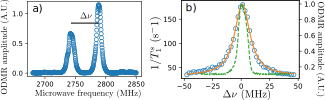
\includegraphics[width=0.45\textwidth]{Figures/fig largeur fluct}
\caption{Modification of the stretch lifetime for two near-resonant classes. (a) ODMR spectrum with amplitude modulation of the microwave for the $\ket{0} \to \ket{-1}$ transition of two separate NV classes. The frequency detuning between the two transitions is denoted $\Delta \nu$. (b) Stretch part of the lifetime decay for one of the two classes as function of the frequency detuning (blue circles), fitted by a Lorentzian with half width at half maximum 8.04 MHz . Green dashed line correspond to the ODMR width of a single class stretched by a factor $\sqrt 2$, approximating the overlap of the two classes (see SI).}
\end{figure}

\begin{figure}
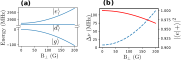
\includegraphics[width=0.45\textwidth]{Figures/fig transverse field simu}
\caption{Simulated eigenstates of the spin Hamiltonian in the presence of purely transverse magnetic field. (a) Energies of the three eigenstates $\ket{g}$, $\ket{d}$ and $\ket{e}$ as a function of the magnetic field amplitude. (b) Blue dashed curve : frequency detuning between the two transitions $\ket{g} \leftrightarrow \ket{d}$ and $\ket{g} \leftrightarrow \ket{e}$. Plain red curve : projection of $\ket{e}$ on $\ket{+}=(\ket{+1}+\ket{-1})/\sqrt{2}$ as a function the magnetic field. Is equal to the projection of $\ket{g}$ on $\ket{0}$.}
\end{figure}

\begin{figure}
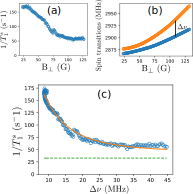
\includegraphics[width=0.45\textwidth]{Figures/fig transverse field}
\caption{Modification of the stretch lifetime in the presence of purely transverse magnetic field. (a) Stretch component of the ensemble lifetime as a function of the field amplitude. (b) Measured transition frequencies through ODMR spectrum. (c) Stretch component of the lifetime as a function of the frequency detuning between the two transistions (blue circles), fitted by a Lorentzian centered in $\Delta \nu=0$ with half width at half maximum 8MHz. The green dashed line correspond to the lifetime of a single class aligned with the magnetic field.}
\end{figure}

\section*{acknowledgements}


\bibliography{CR}



\end{document}